\documentclass[1p]{elsarticle_modified}
%\bibliographystyle{elsarticle-num}

%\usepackage[colorlinks]{hyperref}
%\usepackage{abbrmath_seonhwa} %\Abb, \Ascr, \Acal ,\Abf, \Afrak
\usepackage{amsfonts}
\usepackage{amssymb}
\usepackage{amsmath}
\usepackage{amsthm}
\usepackage{scalefnt}
\usepackage{amsbsy}
\usepackage{kotex}
\usepackage{caption}
\usepackage{subfig}
\usepackage{color}
\usepackage{graphicx}
\usepackage{xcolor} %% white, black, red, green, blue, cyan, magenta, yellow
\usepackage{float}
\usepackage{setspace}
\usepackage{hyperref}

\usepackage{tikz}
\usetikzlibrary{arrows}

\usepackage{multirow}
\usepackage{array} % fixed length table
\usepackage{hhline}

%%%%%%%%%%%%%%%%%%%%%
\makeatletter
\renewcommand*\env@matrix[1][\arraystretch]{%
	\edef\arraystretch{#1}%
	\hskip -\arraycolsep
	\let\@ifnextchar\new@ifnextchar
	\array{*\c@MaxMatrixCols c}}
\makeatother %https://tex.stackexchange.com/questions/14071/how-can-i-increase-the-line-spacing-in-a-matrix
%%%%%%%%%%%%%%%

\usepackage[normalem]{ulem}

\newcommand{\msout}[1]{\ifmmode\text{\sout{\ensuremath{#1}}}\else\sout{#1}\fi}
%SOURCE: \msout is \stkout macro in https://tex.stackexchange.com/questions/20609/strikeout-in-math-mode

\newcommand{\cancel}[1]{
	\ifmmode
	{\color{red}\msout{#1}}
	\else
	{\color{red}\sout{#1}}
	\fi
}

\newcommand{\add}[1]{
	{\color{blue}\uwave{#1}}
}

\newcommand{\replace}[2]{
	\ifmmode
	{\color{red}\msout{#1}}{\color{blue}\uwave{#2}}
	\else
	{\color{red}\sout{#1}}{\color{blue}\uwave{#2}}
	\fi
}

\newcommand{\Sol}{\mathcal{S}} %segment
\newcommand{\D}{D} %diagram
\newcommand{\A}{\mathcal{A}} %arc


%%%%%%%%%%%%%%%%%%%%%%%%%%%%%5 test

\def\sl{\operatorname{\textup{SL}}(2,\Cbb)}
\def\psl{\operatorname{\textup{PSL}}(2,\Cbb)}
\def\quan{\mkern 1mu \triangleright \mkern 1mu}

\theoremstyle{definition}
\newtheorem{thm}{Theorem}[section]
\newtheorem{prop}[thm]{Proposition}
\newtheorem{lem}[thm]{Lemma}
\newtheorem{ques}[thm]{Question}
\newtheorem{cor}[thm]{Corollary}
\newtheorem{defn}[thm]{Definition}
\newtheorem{exam}[thm]{Example}
\newtheorem{rmk}[thm]{Remark}
\newtheorem{alg}[thm]{Algorithm}

\newcommand{\I}{\sqrt{-1}}
\begin{document}

%\begin{frontmatter}
%
%\title{Boundary parabolic representations of knots up to 8 crossings}
%
%%% Group authors per affiliation:
%\author{Yunhi Cho} 
%\address{Department of Mathematics, University of Seoul, Seoul, Korea}
%\ead{yhcho@uos.ac.kr}
%
%
%\author{Seonhwa Kim} %\fnref{s_kim}}
%\address{Center for Geometry and Physics, Institute for Basic Science, Pohang, 37673, Korea}
%\ead{ryeona17@ibs.re.kr}
%
%\author{Hyuk Kim}
%\address{Department of Mathematical Sciences, Seoul National University, Seoul 08826, Korea}
%\ead{hyukkim@snu.ac.kr}
%
%\author{Seokbeom Yoon}
%\address{Department of Mathematical Sciences, Seoul National University, Seoul, 08826,  Korea}
%\ead{sbyoon15@snu.ac.kr}
%
%\begin{abstract}
%We find all boundary parabolic representation of knots up to 8 crossings.
%
%\end{abstract}
%\begin{keyword}
%    \MSC[2010] 57M25 
%\end{keyword}
%
%\end{frontmatter}

%\linenumbers
%\tableofcontents
%
\newcommand\colored[1]{\textcolor{white}{\rule[-0.35ex]{0.8em}{1.4ex}}\kern-0.8em\color{red} #1}%
%\newcommand\colored[1]{\textcolor{white}{ #1}\kern-2.17ex	\textcolor{white}{ #1}\kern-1.81ex	\textcolor{white}{ #1}\kern-2.15ex\color{red}#1	}

{\Large $\underline{11a_{314}~(K11a_{314})}$}

\setlength{\tabcolsep}{10pt}
\renewcommand{\arraystretch}{1.6}
\vspace{1cm}\begin{tabular}{m{100pt}>{\centering\arraybackslash}m{274pt}}
\multirow{5}{120pt}{
	\centering
	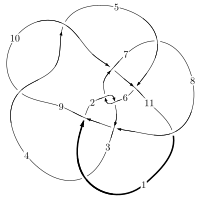
\includegraphics[width=112pt]{../../../GIT/diagram.site/Diagrams/png/563_11a_314.png}\\
\ \ \ A knot diagram\footnotemark}&
\allowdisplaybreaks
\textbf{Linearized knot diagam} \\
\cline{2-2}
 &
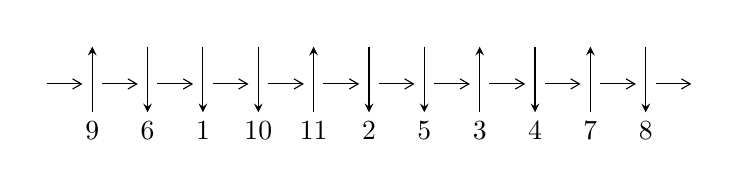
\begin{tikzpicture}[x=20pt, y=17pt]
	% nodes
	\node (C0) at (0, 0) {};
	\node (C1) at (1, 0) {};
	\node (C1U) at (1, +1) {};
	\node (C1D) at (1, -1) {9};

	\node (C2) at (2, 0) {};
	\node (C2U) at (2, +1) {};
	\node (C2D) at (2, -1) {6};

	\node (C3) at (3, 0) {};
	\node (C3U) at (3, +1) {};
	\node (C3D) at (3, -1) {1};

	\node (C4) at (4, 0) {};
	\node (C4U) at (4, +1) {};
	\node (C4D) at (4, -1) {10};

	\node (C5) at (5, 0) {};
	\node (C5U) at (5, +1) {};
	\node (C5D) at (5, -1) {11};

	\node (C6) at (6, 0) {};
	\node (C6U) at (6, +1) {};
	\node (C6D) at (6, -1) {2};

	\node (C7) at (7, 0) {};
	\node (C7U) at (7, +1) {};
	\node (C7D) at (7, -1) {5};

	\node (C8) at (8, 0) {};
	\node (C8U) at (8, +1) {};
	\node (C8D) at (8, -1) {3};

	\node (C9) at (9, 0) {};
	\node (C9U) at (9, +1) {};
	\node (C9D) at (9, -1) {4};

	\node (C10) at (10, 0) {};
	\node (C10U) at (10, +1) {};
	\node (C10D) at (10, -1) {7};

	\node (C11) at (11, 0) {};
	\node (C11U) at (11, +1) {};
	\node (C11D) at (11, -1) {8};
	\node (C12) at (12, 0) {};

	% arrows
	\draw[->,>={angle 60}]
	(C0) edge (C1) (C1) edge (C2) (C2) edge (C3) (C3) edge (C4) (C4) edge (C5) (C5) edge (C6) (C6) edge (C7) (C7) edge (C8) (C8) edge (C9) (C9) edge (C10) (C10) edge (C11) (C11) edge (C12) ;	\draw[->,>=stealth]
	(C1D) edge (C1U) (C2U) edge (C2D) (C3U) edge (C3D) (C4U) edge (C4D) (C5D) edge (C5U) (C6U) edge (C6D) (C7U) edge (C7D) (C8D) edge (C8U) (C9U) edge (C9D) (C10D) edge (C10U) (C11U) edge (C11D) ;
	\end{tikzpicture} \\
\hhline{~~} \\& 
\textbf{Solving Sequence} \\ \cline{2-2} 
 &
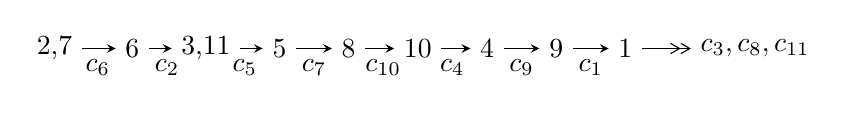
\begin{tikzpicture}[x=25pt, y=7pt]
	% node
	\node (A0) at (-1/8, 0) {2,7};
	\node (A1) at (1, 0) {6};
	\node (A2) at (33/16, 0) {3,11};
	\node (A3) at (25/8, 0) {5};
	\node (A4) at (33/8, 0) {8};
	\node (A5) at (41/8, 0) {10};
	\node (A6) at (49/8, 0) {4};
	\node (A7) at (57/8, 0) {9};
	\node (A8) at (65/8, 0) {1};
	\node (C1) at (1/2, -1) {$c_{6}$};
	\node (C2) at (3/2, -1) {$c_{2}$};
	\node (C3) at (21/8, -1) {$c_{5}$};
	\node (C4) at (29/8, -1) {$c_{7}$};
	\node (C5) at (37/8, -1) {$c_{10}$};
	\node (C6) at (45/8, -1) {$c_{4}$};
	\node (C7) at (53/8, -1) {$c_{9}$};
	\node (C8) at (61/8, -1) {$c_{1}$};
	\node (A9) at (10, 0) {$c_{3},c_{8},c_{11}$};

	% edge
	\draw[->,>=stealth]	
	(A0) edge (A1) (A1) edge (A2) (A2) edge (A3) (A3) edge (A4) (A4) edge (A5) (A5) edge (A6) (A6) edge (A7) (A7) edge (A8) ;
	\draw[->>,>={angle 60}]	
	(A8) edge (A9);
\end{tikzpicture} \\ 

\end{tabular} \\

\footnotetext{
The image of knot diagram is generated by the software ``\textbf{Draw programme}" developed by Andrew Bartholomew(\url{http://www.layer8.co.uk/maths/draw/index.htm\#Running-draw}), where we modified some parts for our purpose(\url{https://github.com/CATsTAILs/LinksPainter}).
}\phantom \\ \newline 
\centering \textbf{Ideals for irreducible components\footnotemark of $X_{\text{par}}$} 
 
\begin{align*}
I^u_{1}&=\langle 
8.61471\times10^{40} u^{35}-1.83411\times10^{41} u^{34}+\cdots+5.25231\times10^{41} b-3.70395\times10^{41},\\
\phantom{I^u_{1}}&\phantom{= \langle  }2.23742\times10^{42} u^{35}-7.36115\times10^{42} u^{34}+\cdots+1.10299\times10^{43} a-4.47196\times10^{43},\;u^{36}-3 u^{35}+\cdots-41 u+8\rangle \\
I^u_{2}&=\langle 
-2.43055\times10^{20} a u^{32}+6.47281\times10^{20} u^{32}+\cdots-3.83637\times10^{20} a-8.61406\times10^{20},\\
\phantom{I^u_{2}}&\phantom{= \langle  }4.95038\times10^{20} a u^{32}-3.49948\times10^{20} u^{32}+\cdots+5.33454\times10^{20} a+1.26914\times10^{21},\;u^{33}+u^{32}+\cdots-2 u-1\rangle \\
I^u_{3}&=\langle 
u^5 a-3 u^4 a-4 u^5+4 u^3 a+3 u^4-2 u^2 a-13 u^3+8 u^2+3 b- a-12 u+1,\\
\phantom{I^u_{3}}&\phantom{= \langle  }21 u^5 a+19 u^5+63 u^3 a-23 u^4+14 u^2 a+72 u^3+7 a^2+42 a u-67 u^2+56 a+80 u-20,\\
\phantom{I^u_{3}}&\phantom{= \langle  }u^6- u^5+4 u^4-3 u^3+5 u^2- u+1\rangle \\
I^u_{4}&=\langle 
- u^3-2 u^2+b-2 u-1,\;u^4+u^3+a- u-2,\;u^5+2 u^4+3 u^3+3 u^2+u+1\rangle \\
\\
\end{align*}
\raggedright * 4 irreducible components of $\dim_{\mathbb{C}}=0$, with total 119 representations.\\
\footnotetext{All coefficients of polynomials are rational numbers. But the coefficients are sometimes approximated in decimal forms when there is not enough margin.}
\newpage
\renewcommand{\arraystretch}{1}
\centering \section*{I. $I^u_{1}= \langle 8.61\times10^{40} u^{35}-1.83\times10^{41} u^{34}+\cdots+5.25\times10^{41} b-3.70\times10^{41},\;2.24\times10^{42} u^{35}-7.36\times10^{42} u^{34}+\cdots+1.10\times10^{43} a-4.47\times10^{43},\;u^{36}-3 u^{35}+\cdots-41 u+8 \rangle$}
\flushleft \textbf{(i) Arc colorings}\\
\begin{tabular}{m{7pt} m{180pt} m{7pt} m{180pt} }
\flushright $a_{2}=$&$\begin{pmatrix}0\\u\end{pmatrix}$ \\
\flushright $a_{7}=$&$\begin{pmatrix}1\\0\end{pmatrix}$ \\
\flushright $a_{6}=$&$\begin{pmatrix}1\\- u^2\end{pmatrix}$ \\
\flushright $a_{3}=$&$\begin{pmatrix}- u\\u^3+u\end{pmatrix}$ \\
\flushright $a_{11}=$&$\begin{pmatrix}-0.202851 u^{35}+0.667384 u^{34}+\cdots-15.2882 u+4.05441\\-0.164017 u^{35}+0.349200 u^{34}+\cdots-2.46540 u+0.705203\end{pmatrix}$ \\
\flushright $a_{5}=$&$\begin{pmatrix}-0.105569 u^{35}+0.356434 u^{34}+\cdots-12.7501 u+5.10427\\-0.226388 u^{35}+0.544294 u^{34}+\cdots-6.01564 u+1.25342\end{pmatrix}$ \\
\flushright $a_{8}=$&$\begin{pmatrix}0.00692985 u^{35}-0.108881 u^{34}+\cdots+5.10249 u+0.776589\\0.0935874 u^{35}-0.140600 u^{34}+\cdots-2.26813 u+1.29025\end{pmatrix}$ \\
\flushright $a_{10}=$&$\begin{pmatrix}-0.0388338 u^{35}+0.318184 u^{34}+\cdots-12.8228 u+3.34921\\-0.164017 u^{35}+0.349200 u^{34}+\cdots-2.46540 u+0.705203\end{pmatrix}$ \\
\flushright $a_{4}=$&$\begin{pmatrix}-0.103938 u^{35}+0.595414 u^{34}+\cdots-24.0552 u+7.44471\\-0.283599 u^{35}+0.624540 u^{34}+\cdots-3.18323 u-0.831508\end{pmatrix}$ \\
\flushright $a_{9}=$&$\begin{pmatrix}-0.0881504 u^{35}+0.100434 u^{34}+\cdots+3.42966 u+1.14876\\0.201683 u^{35}-0.426849 u^{34}+\cdots+1.75702 u+0.310670\end{pmatrix}$ \\
\flushright $a_{1}=$&$\begin{pmatrix}0.396588 u^{35}-0.858030 u^{34}+\cdots+4.64230 u-0.696871\\-0.354176 u^{35}+0.932845 u^{34}+\cdots-16.5994 u+2.94258\end{pmatrix}$\\ \flushright $a_{1}=$&$\begin{pmatrix}0.396588 u^{35}-0.858030 u^{34}+\cdots+4.64230 u-0.696871\\-0.354176 u^{35}+0.932845 u^{34}+\cdots-16.5994 u+2.94258\end{pmatrix}$\\&\end{tabular}
\flushleft \textbf{(ii) Obstruction class $= -1$}\\~\\
\flushleft \textbf{(iii) Cusp Shapes $= 0.705642 u^{35}-1.36959 u^{34}+\cdots-2.37672 u+0.386803$}\\~\\
\newpage\renewcommand{\arraystretch}{1}
\flushleft \textbf{(iv) u-Polynomials at the component}\newline \\
\begin{tabular}{m{50pt}|m{274pt}}
Crossings & \hspace{64pt}u-Polynomials at each crossing \\
\hline $$\begin{aligned}c_{1},c_{10}\end{aligned}$$&$\begin{aligned}
&u^{36}+2 u^{35}+\cdots-144 u-14
\end{aligned}$\\
\hline $$\begin{aligned}c_{2},c_{6}\end{aligned}$$&$\begin{aligned}
&u^{36}+3 u^{35}+\cdots+41 u+8
\end{aligned}$\\
\hline $$\begin{aligned}c_{3},c_{7}\end{aligned}$$&$\begin{aligned}
&u^{36}- u^{35}+\cdots+u-7
\end{aligned}$\\
\hline $$\begin{aligned}c_{4},c_{9}\end{aligned}$$&$\begin{aligned}
&7(7 u^{36}-27 u^{35}+\cdots-32 u-64)
\end{aligned}$\\
\hline $$\begin{aligned}c_{5},c_{8}\end{aligned}$$&$\begin{aligned}
&7(7 u^{36}-6 u^{35}+\cdots-4 u+1)
\end{aligned}$\\
\hline $$\begin{aligned}c_{11}\end{aligned}$$&$\begin{aligned}
&u^{36}+6 u^{35}+\cdots-2641 u-394
\end{aligned}$\\
\hline
\end{tabular}\\~\\
\newpage\renewcommand{\arraystretch}{1}
\flushleft \textbf{(v) Riley Polynomials at the component}\newline \\
\begin{tabular}{m{50pt}|m{274pt}}
Crossings & \hspace{64pt}Riley Polynomials at each crossing \\
\hline $$\begin{aligned}c_{1},c_{10}\end{aligned}$$&$\begin{aligned}
&y^{36}+2 y^{35}+\cdots-2592 y+196
\end{aligned}$\\
\hline $$\begin{aligned}c_{2},c_{6}\end{aligned}$$&$\begin{aligned}
&y^{36}+13 y^{35}+\cdots-641 y+64
\end{aligned}$\\
\hline $$\begin{aligned}c_{3},c_{7}\end{aligned}$$&$\begin{aligned}
&y^{36}-9 y^{35}+\cdots+321 y+49
\end{aligned}$\\
\hline $$\begin{aligned}c_{4},c_{9}\end{aligned}$$&$\begin{aligned}
&49(49 y^{36}-1289 y^{35}+\cdots-31744 y+4096)
\end{aligned}$\\
\hline $$\begin{aligned}c_{5},c_{8}\end{aligned}$$&$\begin{aligned}
&49(49 y^{36}-456 y^{35}+\cdots-20 y+1)
\end{aligned}$\\
\hline $$\begin{aligned}c_{11}\end{aligned}$$&$\begin{aligned}
&y^{36}+4 y^{35}+\cdots-1886765 y+155236
\end{aligned}$\\
\hline
\end{tabular}\\~\\
\newpage\flushleft \textbf{(vi) Complex Volumes and Cusp Shapes}
$$\begin{array}{c|c|c}  
\text{Solutions to }I^u_{1}& \I (\text{vol} + \sqrt{-1}CS) & \text{Cusp shape}\\
 \hline 
\begin{aligned}
u &= \phantom{-}0.664991 + 0.788504 I \\
a &= \phantom{-}0.206169 - 0.722289 I \\
b &= \phantom{-}0.096578 + 0.477168 I\end{aligned}
 & -1.34782 - 1.56519 I & \phantom{-}0.84439 + 2.92266 I \\ \hline\begin{aligned}
u &= \phantom{-}0.664991 - 0.788504 I \\
a &= \phantom{-}0.206169 + 0.722289 I \\
b &= \phantom{-}0.096578 - 0.477168 I\end{aligned}
 & -1.34782 + 1.56519 I & \phantom{-}0.84439 - 2.92266 I \\ \hline\begin{aligned}
u &= \phantom{-}0.309249 + 0.905547 I \\
a &= \phantom{-}1.79251 + 0.71331 I \\
b &= \phantom{-}0.751216 + 0.448888 I\end{aligned}
 & -1.22381 - 2.38943 I & -2.60962 + 0.88195 I \\ \hline\begin{aligned}
u &= \phantom{-}0.309249 - 0.905547 I \\
a &= \phantom{-}1.79251 - 0.71331 I \\
b &= \phantom{-}0.751216 - 0.448888 I\end{aligned}
 & -1.22381 + 2.38943 I & -2.60962 - 0.88195 I \\ \hline\begin{aligned}
u &= -0.888722 + 0.321374 I \\
a &= \phantom{-}0.363466 - 0.084941 I \\
b &= \phantom{-}0.703627 - 0.796093 I\end{aligned}
 & -1.32711 - 7.08620 I & -4.38282 + 7.74538 I \\ \hline\begin{aligned}
u &= -0.888722 - 0.321374 I \\
a &= \phantom{-}0.363466 + 0.084941 I \\
b &= \phantom{-}0.703627 + 0.796093 I\end{aligned}
 & -1.32711 + 7.08620 I & -4.38282 - 7.74538 I \\ \hline\begin{aligned}
u &= -0.518925 + 1.036550 I \\
a &= -0.767941 + 0.827823 I \\
b &= -1.051610 + 0.091581 I\end{aligned}
 & \phantom{-}3.19944 + 1.84265 I & \phantom{-}5.26933 - 1.44076 I \\ \hline\begin{aligned}
u &= -0.518925 - 1.036550 I \\
a &= -0.767941 - 0.827823 I \\
b &= -1.051610 - 0.091581 I\end{aligned}
 & \phantom{-}3.19944 - 1.84265 I & \phantom{-}5.26933 + 1.44076 I \\ \hline\begin{aligned}
u &= -1.16822\phantom{ +0.000000I} \\
a &= -0.710710\phantom{ +0.000000I} \\
b &= \phantom{-}0.650117\phantom{ +0.000000I}\end{aligned}
 & -7.32636\phantom{ +0.000000I} & -13.3830\phantom{ +0.000000I} \\ \hline\begin{aligned}
u &= \phantom{-}0.478238 + 1.066020 I \\
a &= \phantom{-}2.08338 + 0.02701 I \\
b &= \phantom{-}0.97824 - 1.76146 I\end{aligned}
 & -0.67631 - 8.62575 I & \phantom{-}0.85500 + 10.45337 I\\
 \hline 
 \end{array}$$\newpage$$\begin{array}{c|c|c}  
\text{Solutions to }I^u_{1}& \I (\text{vol} + \sqrt{-1}CS) & \text{Cusp shape}\\
 \hline 
\begin{aligned}
u &= \phantom{-}0.478238 - 1.066020 I \\
a &= \phantom{-}2.08338 - 0.02701 I \\
b &= \phantom{-}0.97824 + 1.76146 I\end{aligned}
 & -0.67631 + 8.62575 I & \phantom{-}0.85500 - 10.45337 I \\ \hline\begin{aligned}
u &= \phantom{-}0.398028 + 1.136150 I \\
a &= \phantom{-}0.553917 + 0.951098 I \\
b &= \phantom{-}1.25000 + 0.81047 I\end{aligned}
 & -0.316044 + 1.377840 I & \phantom{-}0.40549 - 3.04607 I \\ \hline\begin{aligned}
u &= \phantom{-}0.398028 - 1.136150 I \\
a &= \phantom{-}0.553917 - 0.951098 I \\
b &= \phantom{-}1.25000 - 0.81047 I\end{aligned}
 & -0.316044 - 1.377840 I & \phantom{-}0.40549 + 3.04607 I \\ \hline\begin{aligned}
u &= -0.420762 + 1.153070 I \\
a &= -1.70439 + 0.18358 I \\
b &= -1.14723 - 1.04061 I\end{aligned}
 & \phantom{-}3.76935 + 5.55914 I & \phantom{-}7.29930 - 8.75003 I \\ \hline\begin{aligned}
u &= -0.420762 - 1.153070 I \\
a &= -1.70439 - 0.18358 I \\
b &= -1.14723 + 1.04061 I\end{aligned}
 & \phantom{-}3.76935 - 5.55914 I & \phantom{-}7.29930 + 8.75003 I \\ \hline\begin{aligned}
u &= \phantom{-}1.22770\phantom{ +0.000000I} \\
a &= \phantom{-}0.220807\phantom{ +0.000000I} \\
b &= \phantom{-}0.272974\phantom{ +0.000000I}\end{aligned}
 & -2.30591\phantom{ +0.000000I} & -25.6820\phantom{ +0.000000I} \\ \hline\begin{aligned}
u &= \phantom{-}0.773847 + 1.014680 I \\
a &= \phantom{-}0.823733 + 0.526895 I \\
b &= \phantom{-}0.348098 - 0.539202 I\end{aligned}
 & -0.76840 - 4.07443 I & -2.61964 + 5.42418 I \\ \hline\begin{aligned}
u &= \phantom{-}0.773847 - 1.014680 I \\
a &= \phantom{-}0.823733 - 0.526895 I \\
b &= \phantom{-}0.348098 + 0.539202 I\end{aligned}
 & -0.76840 + 4.07443 I & -2.61964 - 5.42418 I \\ \hline\begin{aligned}
u &= \phantom{-}1.213610 + 0.471997 I \\
a &= \phantom{-}0.0522347 + 0.0634017 I \\
b &= -0.99435 - 1.13172 I\end{aligned}
 & -7.25713 + 12.05490 I & -6.87385 - 7.36867 I \\ \hline\begin{aligned}
u &= \phantom{-}1.213610 - 0.471997 I \\
a &= \phantom{-}0.0522347 - 0.0634017 I \\
b &= -0.99435 + 1.13172 I\end{aligned}
 & -7.25713 - 12.05490 I & -6.87385 + 7.36867 I\\
 \hline 
 \end{array}$$\newpage$$\begin{array}{c|c|c}  
\text{Solutions to }I^u_{1}& \I (\text{vol} + \sqrt{-1}CS) & \text{Cusp shape}\\
 \hline 
\begin{aligned}
u &= -0.611418 + 1.156610 I \\
a &= \phantom{-}1.75019 - 0.34229 I \\
b &= \phantom{-}0.948743 + 0.849128 I\end{aligned}
 & \phantom{-}1.15223 + 12.56020 I & -2.14661 - 10.43699 I \\ \hline\begin{aligned}
u &= -0.611418 - 1.156610 I \\
a &= \phantom{-}1.75019 + 0.34229 I \\
b &= \phantom{-}0.948743 - 0.849128 I\end{aligned}
 & \phantom{-}1.15223 - 12.56020 I & -2.14661 + 10.43699 I \\ \hline\begin{aligned}
u &= -0.096544 + 1.309750 I \\
a &= \phantom{-}1.024940 - 0.533084 I \\
b &= \phantom{-}0.729584 - 0.253643 I\end{aligned}
 & \phantom{-}4.46757 - 3.67706 I & \phantom{-}3.45782 + 3.48358 I \\ \hline\begin{aligned}
u &= -0.096544 - 1.309750 I \\
a &= \phantom{-}1.024940 + 0.533084 I \\
b &= \phantom{-}0.729584 + 0.253643 I\end{aligned}
 & \phantom{-}4.46757 + 3.67706 I & \phantom{-}3.45782 - 3.48358 I \\ \hline\begin{aligned}
u &= \phantom{-}0.556045 + 0.380280 I \\
a &= \phantom{-}0.75859 + 1.37452 I \\
b &= \phantom{-}0.611800 - 1.101080 I\end{aligned}
 & -2.98357 - 5.46509 I & -4.40298 + 5.74809 I \\ \hline\begin{aligned}
u &= \phantom{-}0.556045 - 0.380280 I \\
a &= \phantom{-}0.75859 - 1.37452 I \\
b &= \phantom{-}0.611800 + 1.101080 I\end{aligned}
 & -2.98357 + 5.46509 I & -4.40298 - 5.74809 I \\ \hline\begin{aligned}
u &= \phantom{-}0.331294 + 0.549198 I \\
a &= -2.03245 + 0.47407 I \\
b &= \phantom{-}0.44966 + 1.55974 I\end{aligned}
 & -2.49638 + 4.90008 I & -3.79310 - 7.77480 I \\ \hline\begin{aligned}
u &= \phantom{-}0.331294 - 0.549198 I \\
a &= -2.03245 - 0.47407 I \\
b &= \phantom{-}0.44966 - 1.55974 I\end{aligned}
 & -2.49638 - 4.90008 I & -3.79310 + 7.77480 I \\ \hline\begin{aligned}
u &= -0.572685 + 0.080761 I \\
a &= \phantom{-}0.472008 - 0.470814 I \\
b &= -0.639767 + 0.652105 I\end{aligned}
 & \phantom{-}0.74933 - 1.67412 I & \phantom{-}0.81111 + 4.63626 I \\ \hline\begin{aligned}
u &= -0.572685 - 0.080761 I \\
a &= \phantom{-}0.472008 + 0.470814 I \\
b &= -0.639767 - 0.652105 I\end{aligned}
 & \phantom{-}0.74933 + 1.67412 I & \phantom{-}0.81111 - 4.63626 I\\
 \hline 
 \end{array}$$\newpage$$\begin{array}{c|c|c}  
\text{Solutions to }I^u_{1}& \I (\text{vol} + \sqrt{-1}CS) & \text{Cusp shape}\\
 \hline 
\begin{aligned}
u &= \phantom{-}0.74631 + 1.24839 I \\
a &= -1.54739 - 0.38151 I \\
b &= -1.09203 + 1.33473 I\end{aligned}
 & -4.7264 - 18.9578 I & -4.99741 + 9.85636 I \\ \hline\begin{aligned}
u &= \phantom{-}0.74631 - 1.24839 I \\
a &= -1.54739 + 0.38151 I \\
b &= -1.09203 - 1.33473 I\end{aligned}
 & -4.7264 + 18.9578 I & -4.99741 - 9.85636 I \\ \hline\begin{aligned}
u &= -0.19922 + 1.64465 I \\
a &= -0.938395 - 0.165870 I \\
b &= -1.27867 - 0.61003 I\end{aligned}
 & \phantom{-}1.57745 + 7.38932 I & \phantom{-0.000000 } 0 \\ \hline\begin{aligned}
u &= -0.19922 - 1.64465 I \\
a &= -0.938395 + 0.165870 I \\
b &= -1.27867 + 0.61003 I\end{aligned}
 & \phantom{-}1.57745 - 7.38932 I & \phantom{-0.000000 } 0 \\ \hline\begin{aligned}
u &= \phantom{-}0.317864\phantom{ +0.000000I} \\
a &= \phantom{-}1.05754\phantom{ +0.000000I} \\
b &= \phantom{-}0.804397\phantom{ +0.000000I}\end{aligned}
 & -3.24067\phantom{ +0.000000I} & -2.80810\phantom{ +0.000000I} \\ \hline\begin{aligned}
u &= -1.70401\phantom{ +0.000000I} \\
a &= \phantom{-}0.0619210\phantom{ +0.000000I} \\
b &= -1.05525\phantom{ +0.000000I}\end{aligned}
 & -5.25552\phantom{ +0.000000I} & \phantom{-0.000000 } 0\\
 \hline 
 \end{array}$$\newpage\newpage\renewcommand{\arraystretch}{1}
\centering \section*{II. $I^u_{2}= \langle -2.43\times10^{20} a u^{32}+6.47\times10^{20} u^{32}+\cdots-3.84\times10^{20} a-8.61\times10^{20},\;4.95\times10^{20} a u^{32}-3.50\times10^{20} u^{32}+\cdots+5.33\times10^{20} a+1.27\times10^{21},\;u^{33}+u^{32}+\cdots-2 u-1 \rangle$}
\flushleft \textbf{(i) Arc colorings}\\
\begin{tabular}{m{7pt} m{180pt} m{7pt} m{180pt} }
\flushright $a_{2}=$&$\begin{pmatrix}0\\u\end{pmatrix}$ \\
\flushright $a_{7}=$&$\begin{pmatrix}1\\0\end{pmatrix}$ \\
\flushright $a_{6}=$&$\begin{pmatrix}1\\- u^2\end{pmatrix}$ \\
\flushright $a_{3}=$&$\begin{pmatrix}- u\\u^3+u\end{pmatrix}$ \\
\flushright $a_{11}=$&$\begin{pmatrix}a\\6.17561 a u^{32}-16.4463 u^{32}+\cdots+9.74756 a+21.8868\end{pmatrix}$ \\
\flushright $a_{5}=$&$\begin{pmatrix}15.4244 a u^{32}+18.6669 u^{32}+\cdots-21.4494 a+11.7346\\-2.41747 a u^{32}-4.89104 u^{32}+\cdots+4.36925 a+5.31631\end{pmatrix}$ \\
\flushright $a_{8}=$&$\begin{pmatrix}-20.3325 a u^{32}-29.5888 u^{32}+\cdots+30.2366 a+1.23756\\-1.92091 a u^{32}+11.7466 u^{32}+\cdots-5.00243 a-20.0640\end{pmatrix}$ \\
\flushright $a_{10}=$&$\begin{pmatrix}-6.17561 a u^{32}+16.4463 u^{32}+\cdots-8.74756 a-21.8868\\6.17561 a u^{32}-16.4463 u^{32}+\cdots+9.74756 a+21.8868\end{pmatrix}$ \\
\flushright $a_{4}=$&$\begin{pmatrix}8.00399 a u^{32}+35.7108 u^{32}+\cdots-26.8856 a-24.1021\\9.29658 a u^{32}-21.9349 u^{32}+\cdots+8.00399 a+41.1530\end{pmatrix}$ \\
\flushright $a_{9}=$&$\begin{pmatrix}-9.74756 a u^{32}-30.4209 u^{32}+\cdots+24.0610 a+16.6620\\-10.5850 a u^{32}+5.09705 u^{32}+\cdots+6.17561 a-27.2965\end{pmatrix}$ \\
\flushright $a_{1}=$&$\begin{pmatrix}0.494744 a u^{32}+24.1111 u^{32}+\cdots-16.2512 a-28.9205\\11.8477 a u^{32}-13.2154 u^{32}+\cdots+5.90658 a+35.7744\end{pmatrix}$\\ \flushright $a_{1}=$&$\begin{pmatrix}0.494744 a u^{32}+24.1111 u^{32}+\cdots-16.2512 a-28.9205\\11.8477 a u^{32}-13.2154 u^{32}+\cdots+5.90658 a+35.7744\end{pmatrix}$\\&\end{tabular}
\flushleft \textbf{(ii) Obstruction class $= -1$}\\~\\
\flushleft \textbf{(iii) Cusp Shapes $= -\frac{233960085812908682097}{13119091879006586663} u^{32}-\frac{122838803537233845053}{39357275637019759989} u^{31}+\cdots-\frac{1020433678799244188345}{39357275637019759989} u-\frac{1174252898466954031738}{39357275637019759989}$}\\~\\
\newpage\renewcommand{\arraystretch}{1}
\flushleft \textbf{(iv) u-Polynomials at the component}\newline \\
\begin{tabular}{m{50pt}|m{274pt}}
Crossings & \hspace{64pt}u-Polynomials at each crossing \\
\hline $$\begin{aligned}c_{1},c_{10}\end{aligned}$$&$\begin{aligned}
&u^{66}- u^{65}+\cdots+360 u+11
\end{aligned}$\\
\hline $$\begin{aligned}c_{2},c_{6}\end{aligned}$$&$\begin{aligned}
&(u^{33}- u^{32}+\cdots-2 u+1)^{2}
\end{aligned}$\\
\hline $$\begin{aligned}c_{3},c_{7}\end{aligned}$$&$\begin{aligned}
&u^{66}-11 u^{65}+\cdots-3027 u+484
\end{aligned}$\\
\hline $$\begin{aligned}c_{4},c_{9}\end{aligned}$$&$\begin{aligned}
&(u^{33}-13 u^{31}+\cdots+60 u+9)^{2}
\end{aligned}$\\
\hline $$\begin{aligned}c_{5},c_{8}\end{aligned}$$&$\begin{aligned}
&u^{66}+2 u^{65}+\cdots-9 u+2
\end{aligned}$\\
\hline $$\begin{aligned}c_{11}\end{aligned}$$&$\begin{aligned}
&(u^{33}-5 u^{32}+\cdots+88 u-47)^{2}
\end{aligned}$\\
\hline
\end{tabular}\\~\\
\newpage\renewcommand{\arraystretch}{1}
\flushleft \textbf{(v) Riley Polynomials at the component}\newline \\
\begin{tabular}{m{50pt}|m{274pt}}
Crossings & \hspace{64pt}Riley Polynomials at each crossing \\
\hline $$\begin{aligned}c_{1},c_{10}\end{aligned}$$&$\begin{aligned}
&y^{66}+25 y^{65}+\cdots-60564 y+121
\end{aligned}$\\
\hline $$\begin{aligned}c_{2},c_{6}\end{aligned}$$&$\begin{aligned}
&(y^{33}+21 y^{32}+\cdots-20 y-1)^{2}
\end{aligned}$\\
\hline $$\begin{aligned}c_{3},c_{7}\end{aligned}$$&$\begin{aligned}
&y^{66}-29 y^{65}+\cdots-9905185 y+234256
\end{aligned}$\\
\hline $$\begin{aligned}c_{4},c_{9}\end{aligned}$$&$\begin{aligned}
&(y^{33}-26 y^{32}+\cdots+828 y-81)^{2}
\end{aligned}$\\
\hline $$\begin{aligned}c_{5},c_{8}\end{aligned}$$&$\begin{aligned}
&y^{66}+28 y^{65}+\cdots-41 y+4
\end{aligned}$\\
\hline $$\begin{aligned}c_{11}\end{aligned}$$&$\begin{aligned}
&(y^{33}-23 y^{32}+\cdots+24852 y-2209)^{2}
\end{aligned}$\\
\hline
\end{tabular}\\~\\
\newpage\flushleft \textbf{(vi) Complex Volumes and Cusp Shapes}
$$\begin{array}{c|c|c}  
\text{Solutions to }I^u_{2}& \I (\text{vol} + \sqrt{-1}CS) & \text{Cusp shape}\\
 \hline 
\begin{aligned}
u &= -0.417392 + 0.929081 I \\
a &= \phantom{-}0.117806 - 1.017110 I \\
b &= \phantom{-}0.61426 - 1.45227 I\end{aligned}
 & -0.35121 + 5.74395 I & -4.00846 - 9.48122 I \\ \hline\begin{aligned}
u &= -0.417392 + 0.929081 I \\
a &= -2.40309 + 0.13570 I \\
b &= -0.476485 - 0.850411 I\end{aligned}
 & -0.35121 + 5.74395 I & -4.00846 - 9.48122 I \\ \hline\begin{aligned}
u &= -0.417392 - 0.929081 I \\
a &= \phantom{-}0.117806 + 1.017110 I \\
b &= \phantom{-}0.61426 + 1.45227 I\end{aligned}
 & -0.35121 - 5.74395 I & -4.00846 + 9.48122 I \\ \hline\begin{aligned}
u &= -0.417392 - 0.929081 I \\
a &= -2.40309 - 0.13570 I \\
b &= -0.476485 + 0.850411 I\end{aligned}
 & -0.35121 - 5.74395 I & -4.00846 + 9.48122 I \\ \hline\begin{aligned}
u &= \phantom{-}0.414454 + 0.869237 I \\
a &= -0.900638 + 0.750691 I \\
b &= -0.465090 - 0.778291 I\end{aligned}
 & -0.30625 - 1.73487 I & -2.88654 + 2.20347 I \\ \hline\begin{aligned}
u &= \phantom{-}0.414454 + 0.869237 I \\
a &= -2.65339 - 0.05663 I \\
b &= -0.671706 + 0.442842 I\end{aligned}
 & -0.30625 - 1.73487 I & -2.88654 + 2.20347 I \\ \hline\begin{aligned}
u &= \phantom{-}0.414454 - 0.869237 I \\
a &= -0.900638 - 0.750691 I \\
b &= -0.465090 + 0.778291 I\end{aligned}
 & -0.30625 + 1.73487 I & -2.88654 - 2.20347 I \\ \hline\begin{aligned}
u &= \phantom{-}0.414454 - 0.869237 I \\
a &= -2.65339 + 0.05663 I \\
b &= -0.671706 - 0.442842 I\end{aligned}
 & -0.30625 + 1.73487 I & -2.88654 - 2.20347 I \\ \hline\begin{aligned}
u &= -0.472417 + 1.010790 I \\
a &= -1.61213 + 0.10091 I \\
b &= -0.036980 - 0.568939 I\end{aligned}
 & -4.16587 + 3.01159 I & -11.51158 - 5.38736 I \\ \hline\begin{aligned}
u &= -0.472417 + 1.010790 I \\
a &= \phantom{-}2.01812 - 0.47306 I \\
b &= \phantom{-}1.80069 + 1.09379 I\end{aligned}
 & -4.16587 + 3.01159 I & -11.51158 - 5.38736 I\\
 \hline 
 \end{array}$$\newpage$$\begin{array}{c|c|c}  
\text{Solutions to }I^u_{2}& \I (\text{vol} + \sqrt{-1}CS) & \text{Cusp shape}\\
 \hline 
\begin{aligned}
u &= -0.472417 - 1.010790 I \\
a &= -1.61213 - 0.10091 I \\
b &= -0.036980 + 0.568939 I\end{aligned}
 & -4.16587 - 3.01159 I & -11.51158 + 5.38736 I \\ \hline\begin{aligned}
u &= -0.472417 - 1.010790 I \\
a &= \phantom{-}2.01812 + 0.47306 I \\
b &= \phantom{-}1.80069 - 1.09379 I\end{aligned}
 & -4.16587 - 3.01159 I & -11.51158 + 5.38736 I \\ \hline\begin{aligned}
u &= \phantom{-}0.100593 + 1.216160 I \\
a &= \phantom{-}1.33835 + 0.55468 I \\
b &= \phantom{-}0.808856 + 0.245405 I\end{aligned}
 & \phantom{-}4.81646 - 2.61267 I & \phantom{-}2.98003 + 2.49183 I \\ \hline\begin{aligned}
u &= \phantom{-}0.100593 + 1.216160 I \\
a &= -1.41971 + 0.56060 I \\
b &= -1.094700 + 0.741598 I\end{aligned}
 & \phantom{-}4.81646 - 2.61267 I & \phantom{-}2.98003 + 2.49183 I \\ \hline\begin{aligned}
u &= \phantom{-}0.100593 - 1.216160 I \\
a &= \phantom{-}1.33835 - 0.55468 I \\
b &= \phantom{-}0.808856 - 0.245405 I\end{aligned}
 & \phantom{-}4.81646 + 2.61267 I & \phantom{-}2.98003 - 2.49183 I \\ \hline\begin{aligned}
u &= \phantom{-}0.100593 - 1.216160 I \\
a &= -1.41971 - 0.56060 I \\
b &= -1.094700 - 0.741598 I\end{aligned}
 & \phantom{-}4.81646 + 2.61267 I & \phantom{-}2.98003 - 2.49183 I \\ \hline\begin{aligned}
u &= -0.392936 + 0.664924 I \\
a &= \phantom{-}0.193117 - 0.538220 I \\
b &= -0.344357 + 1.111940 I\end{aligned}
 & -1.06351 - 2.23250 I & -4.94311 + 2.28132 I \\ \hline\begin{aligned}
u &= -0.392936 + 0.664924 I \\
a &= \phantom{-}1.58119 + 0.03868 I \\
b &= \phantom{-}0.675409 + 0.632548 I\end{aligned}
 & -1.06351 - 2.23250 I & -4.94311 + 2.28132 I \\ \hline\begin{aligned}
u &= -0.392936 - 0.664924 I \\
a &= \phantom{-}0.193117 + 0.538220 I \\
b &= -0.344357 - 1.111940 I\end{aligned}
 & -1.06351 + 2.23250 I & -4.94311 - 2.28132 I \\ \hline\begin{aligned}
u &= -0.392936 - 0.664924 I \\
a &= \phantom{-}1.58119 - 0.03868 I \\
b &= \phantom{-}0.675409 - 0.632548 I\end{aligned}
 & -1.06351 + 2.23250 I & -4.94311 - 2.28132 I\\
 \hline 
 \end{array}$$\newpage$$\begin{array}{c|c|c}  
\text{Solutions to }I^u_{2}& \I (\text{vol} + \sqrt{-1}CS) & \text{Cusp shape}\\
 \hline 
\begin{aligned}
u &= -0.557709 + 1.097620 I \\
a &= -0.260077 + 0.915977 I \\
b &= -0.154095 - 1.041730 I\end{aligned}
 & -5.04427 + 9.67271 I & -8.11986 - 8.22619 I \\ \hline\begin{aligned}
u &= -0.557709 + 1.097620 I \\
a &= \phantom{-}1.93591 - 0.15684 I \\
b &= \phantom{-}1.09058 + 1.15805 I\end{aligned}
 & -5.04427 + 9.67271 I & -8.11986 - 8.22619 I \\ \hline\begin{aligned}
u &= -0.557709 - 1.097620 I \\
a &= -0.260077 - 0.915977 I \\
b &= -0.154095 + 1.041730 I\end{aligned}
 & -5.04427 - 9.67271 I & -8.11986 + 8.22619 I \\ \hline\begin{aligned}
u &= -0.557709 - 1.097620 I \\
a &= \phantom{-}1.93591 + 0.15684 I \\
b &= \phantom{-}1.09058 - 1.15805 I\end{aligned}
 & -5.04427 - 9.67271 I & -8.11986 + 8.22619 I \\ \hline\begin{aligned}
u &= -0.412549 + 0.632401 I \\
a &= \phantom{-}0.06708 - 1.54795 I \\
b &= \phantom{-}0.247885 + 0.969351 I\end{aligned}
 & -5.44291 + 0.78188 I & -12.85213 - 1.24354 I \\ \hline\begin{aligned}
u &= -0.412549 + 0.632401 I \\
a &= -0.41241 - 1.69473 I \\
b &= \phantom{-}0.85738 - 1.44035 I\end{aligned}
 & -5.44291 + 0.78188 I & -12.85213 - 1.24354 I \\ \hline\begin{aligned}
u &= -0.412549 - 0.632401 I \\
a &= \phantom{-}0.06708 + 1.54795 I \\
b &= \phantom{-}0.247885 - 0.969351 I\end{aligned}
 & -5.44291 - 0.78188 I & -12.85213 + 1.24354 I \\ \hline\begin{aligned}
u &= -0.412549 - 0.632401 I \\
a &= -0.41241 + 1.69473 I \\
b &= \phantom{-}0.85738 + 1.44035 I\end{aligned}
 & -5.44291 - 0.78188 I & -12.85213 + 1.24354 I \\ \hline\begin{aligned}
u &= \phantom{-}0.355820 + 0.662489 I \\
a &= \phantom{-}1.360960 - 0.272301 I \\
b &= \phantom{-}0.444016 - 0.015311 I\end{aligned}
 & -0.93123 - 1.60031 I & -4.00690 + 5.61012 I \\ \hline\begin{aligned}
u &= \phantom{-}0.355820 + 0.662489 I \\
a &= \phantom{-}0.518884 - 0.139240 I \\
b &= \phantom{-}0.020761 + 0.794705 I\end{aligned}
 & -0.93123 - 1.60031 I & -4.00690 + 5.61012 I\\
 \hline 
 \end{array}$$\newpage$$\begin{array}{c|c|c}  
\text{Solutions to }I^u_{2}& \I (\text{vol} + \sqrt{-1}CS) & \text{Cusp shape}\\
 \hline 
\begin{aligned}
u &= \phantom{-}0.355820 - 0.662489 I \\
a &= \phantom{-}1.360960 + 0.272301 I \\
b &= \phantom{-}0.444016 + 0.015311 I\end{aligned}
 & -0.93123 + 1.60031 I & -4.00690 - 5.61012 I \\ \hline\begin{aligned}
u &= \phantom{-}0.355820 - 0.662489 I \\
a &= \phantom{-}0.518884 + 0.139240 I \\
b &= \phantom{-}0.020761 - 0.794705 I\end{aligned}
 & -0.93123 + 1.60031 I & -4.00690 - 5.61012 I \\ \hline\begin{aligned}
u &= \phantom{-}0.498996 + 1.149370 I \\
a &= -0.38658 - 1.38128 I \\
b &= -1.85663 - 1.80445 I\end{aligned}
 & -3.63632 - 8.62361 I & -12.3273 + 8.9713 I \\ \hline\begin{aligned}
u &= \phantom{-}0.498996 + 1.149370 I \\
a &= \phantom{-}1.90689 - 0.02871 I \\
b &= \phantom{-}0.79240 - 1.24669 I\end{aligned}
 & -3.63632 - 8.62361 I & -12.3273 + 8.9713 I \\ \hline\begin{aligned}
u &= \phantom{-}0.498996 - 1.149370 I \\
a &= -0.38658 + 1.38128 I \\
b &= -1.85663 + 1.80445 I\end{aligned}
 & -3.63632 + 8.62361 I & -12.3273 - 8.9713 I \\ \hline\begin{aligned}
u &= \phantom{-}0.498996 - 1.149370 I \\
a &= \phantom{-}1.90689 + 0.02871 I \\
b &= \phantom{-}0.79240 + 1.24669 I\end{aligned}
 & -3.63632 + 8.62361 I & -12.3273 - 8.9713 I \\ \hline\begin{aligned}
u &= \phantom{-}1.29498\phantom{ +0.000000I} \\
a &= \phantom{-}0.222091\phantom{ +0.000000I} \\
b &= \phantom{-}0.544464\phantom{ +0.000000I}\end{aligned}
 & -2.30187\phantom{ +0.000000I} & -31.9940\phantom{ +0.000000I} \\ \hline\begin{aligned}
u &= \phantom{-}1.29498\phantom{ +0.000000I} \\
a &= \phantom{-}0.181714\phantom{ +0.000000I} \\
b &= \phantom{-}0.0439292\phantom{ +0.000000I}\end{aligned}
 & -2.30187\phantom{ +0.000000I} & -31.9940\phantom{ +0.000000I} \\ \hline\begin{aligned}
u &= \phantom{-}0.691384 + 0.062495 I \\
a &= \phantom{-}0.254081 + 0.231283 I \\
b &= \phantom{-}0.467648 - 1.124340 I\end{aligned}
 & -6.68521 - 4.32166 I & -11.81943 + 6.69112 I \\ \hline\begin{aligned}
u &= \phantom{-}0.691384 + 0.062495 I \\
a &= \phantom{-}1.03700 + 2.83810 I \\
b &= -0.961413 - 0.876208 I\end{aligned}
 & -6.68521 - 4.32166 I & -11.81943 + 6.69112 I\\
 \hline 
 \end{array}$$\newpage$$\begin{array}{c|c|c}  
\text{Solutions to }I^u_{2}& \I (\text{vol} + \sqrt{-1}CS) & \text{Cusp shape}\\
 \hline 
\begin{aligned}
u &= \phantom{-}0.691384 - 0.062495 I \\
a &= \phantom{-}0.254081 - 0.231283 I \\
b &= \phantom{-}0.467648 + 1.124340 I\end{aligned}
 & -6.68521 + 4.32166 I & -11.81943 - 6.69112 I \\ \hline\begin{aligned}
u &= \phantom{-}0.691384 - 0.062495 I \\
a &= \phantom{-}1.03700 - 2.83810 I \\
b &= -0.961413 + 0.876208 I\end{aligned}
 & -6.68521 + 4.32166 I & -11.81943 - 6.69112 I \\ \hline\begin{aligned}
u &= -0.601870 + 0.332174 I \\
a &= -0.145333 - 0.282143 I \\
b &= \phantom{-}0.676050 - 1.175820 I\end{aligned}
 & -7.19868 - 4.98844 I & -12.36402 + 2.27839 I \\ \hline\begin{aligned}
u &= -0.601870 + 0.332174 I \\
a &= \phantom{-}2.11833 - 2.52447 I \\
b &= -0.529191 + 0.664200 I\end{aligned}
 & -7.19868 - 4.98844 I & -12.36402 + 2.27839 I \\ \hline\begin{aligned}
u &= -0.601870 - 0.332174 I \\
a &= -0.145333 + 0.282143 I \\
b &= \phantom{-}0.676050 + 1.175820 I\end{aligned}
 & -7.19868 + 4.98844 I & -12.36402 - 2.27839 I \\ \hline\begin{aligned}
u &= -0.601870 - 0.332174 I \\
a &= \phantom{-}2.11833 + 2.52447 I \\
b &= -0.529191 - 0.664200 I\end{aligned}
 & -7.19868 + 4.98844 I & -12.36402 - 2.27839 I \\ \hline\begin{aligned}
u &= \phantom{-}0.626600 + 1.208130 I \\
a &= -0.891596 - 0.208892 I \\
b &= -0.885135 + 0.559574 I\end{aligned}
 & \phantom{-}0.84876 - 6.19552 I & -3.00000 + 7.44126 I \\ \hline\begin{aligned}
u &= \phantom{-}0.626600 + 1.208130 I \\
a &= \phantom{-}1.51704 + 0.31423 I \\
b &= \phantom{-}0.819944 - 0.828069 I\end{aligned}
 & \phantom{-}0.84876 - 6.19552 I & -3.00000 + 7.44126 I \\ \hline\begin{aligned}
u &= \phantom{-}0.626600 - 1.208130 I \\
a &= -0.891596 + 0.208892 I \\
b &= -0.885135 - 0.559574 I\end{aligned}
 & \phantom{-}0.84876 + 6.19552 I & -3.00000 - 7.44126 I \\ \hline\begin{aligned}
u &= \phantom{-}0.626600 - 1.208130 I \\
a &= \phantom{-}1.51704 - 0.31423 I \\
b &= \phantom{-}0.819944 + 0.828069 I\end{aligned}
 & \phantom{-}0.84876 + 6.19552 I & -3.00000 - 7.44126 I\\
 \hline 
 \end{array}$$\newpage$$\begin{array}{c|c|c}  
\text{Solutions to }I^u_{2}& \I (\text{vol} + \sqrt{-1}CS) & \text{Cusp shape}\\
 \hline 
\begin{aligned}
u &= -0.60344 + 1.36253 I \\
a &= -0.300421 - 0.241381 I \\
b &= \phantom{-}0.183626 - 0.365150 I\end{aligned}
 & -3.20813 - 1.17398 I & -16.8881 + 0. I\phantom{ +0.000000I} \\ \hline\begin{aligned}
u &= -0.60344 + 1.36253 I \\
a &= -0.029011 + 0.370695 I \\
b &= -0.98290 + 1.89865 I\end{aligned}
 & -3.20813 - 1.17398 I & -16.8881 + 0. I\phantom{ +0.000000I} \\ \hline\begin{aligned}
u &= -0.60344 - 1.36253 I \\
a &= -0.300421 + 0.241381 I \\
b &= \phantom{-}0.183626 + 0.365150 I\end{aligned}
 & -3.20813 + 1.17398 I & -16.8881 + 0. I\phantom{ +0.000000I} \\ \hline\begin{aligned}
u &= -0.60344 - 1.36253 I \\
a &= -0.029011 - 0.370695 I \\
b &= -0.98290 - 1.89865 I\end{aligned}
 & -3.20813 + 1.17398 I & -16.8881 + 0. I\phantom{ +0.000000I} \\ \hline\begin{aligned}
u &= -0.90200 + 1.23014 I \\
a &= \phantom{-}0.567900 - 0.143956 I \\
b &= \phantom{-}0.233108 + 0.551448 I\end{aligned}
 & -2.85108 + 10.01350 I & \phantom{-0.000000 } 0 \\ \hline\begin{aligned}
u &= -0.90200 + 1.23014 I \\
a &= -1.36302 + 0.57989 I \\
b &= -1.16123 - 1.45442 I\end{aligned}
 & -2.85108 + 10.01350 I & \phantom{-0.000000 } 0 \\ \hline\begin{aligned}
u &= -0.90200 - 1.23014 I \\
a &= \phantom{-}0.567900 + 0.143956 I \\
b &= \phantom{-}0.233108 - 0.551448 I\end{aligned}
 & -2.85108 - 10.01350 I & \phantom{-0.000000 } 0 \\ \hline\begin{aligned}
u &= -0.90200 - 1.23014 I \\
a &= -1.36302 - 0.57989 I \\
b &= -1.16123 + 1.45442 I\end{aligned}
 & -2.85108 - 10.01350 I & \phantom{-0.000000 } 0 \\ \hline\begin{aligned}
u &= -0.050458 + 0.377504 I \\
a &= -0.729840 - 1.049950 I \\
b &= \phantom{-}0.396037 + 1.206410 I\end{aligned}
 & -6.81266 + 4.73250 I & -21.9711 - 14.2148 I \\ \hline\begin{aligned}
u &= -0.050458 + 0.377504 I \\
a &= -9.49427 - 0.72345 I \\
b &= -1.60778 - 0.29179 I\end{aligned}
 & -6.81266 + 4.73250 I & -21.9711 - 14.2148 I\\
 \hline 
 \end{array}$$\newpage$$\begin{array}{c|c|c}  
\text{Solutions to }I^u_{2}& \I (\text{vol} + \sqrt{-1}CS) & \text{Cusp shape}\\
 \hline 
\begin{aligned}
u &= -0.050458 - 0.377504 I \\
a &= -0.729840 + 1.049950 I \\
b &= \phantom{-}0.396037 - 1.206410 I\end{aligned}
 & -6.81266 - 4.73250 I & -21.9711 + 14.2148 I \\ \hline\begin{aligned}
u &= -0.050458 - 0.377504 I \\
a &= -9.49427 + 0.72345 I \\
b &= -1.60778 + 0.29179 I\end{aligned}
 & -6.81266 - 4.73250 I & -21.9711 + 14.2148 I \\ \hline\begin{aligned}
u &= \phantom{-}0.57543 + 1.63125 I \\
a &= -0.238828 - 0.129721 I \\
b &= \phantom{-}0.07358 + 1.85946 I\end{aligned}
 & -2.87513 - 0.70475 I & \phantom{-0.000000 } 0 \\ \hline\begin{aligned}
u &= \phantom{-}0.57543 + 1.63125 I \\
a &= \phantom{-}0.005781 + 0.205594 I \\
b &= \phantom{-}0.231256 + 0.346251 I\end{aligned}
 & -2.87513 - 0.70475 I & \phantom{-0.000000 } 0 \\ \hline\begin{aligned}
u &= \phantom{-}0.57543 - 1.63125 I \\
a &= -0.238828 + 0.129721 I \\
b &= \phantom{-}0.07358 - 1.85946 I\end{aligned}
 & -2.87513 + 0.70475 I & \phantom{-0.000000 } 0 \\ \hline\begin{aligned}
u &= \phantom{-}0.57543 - 1.63125 I \\
a &= \phantom{-}0.005781 - 0.205594 I \\
b &= \phantom{-}0.231256 - 0.346251 I\end{aligned}
 & -2.87513 + 0.70475 I & \phantom{-0.000000 } 0\\
 \hline 
 \end{array}$$\newpage\newpage\renewcommand{\arraystretch}{1}
\centering \section*{III. $I^u_{3}= \langle u^5 a-4 u^5+\cdots- a+1,\;21 u^5 a+19 u^5+\cdots+56 a-20,\;u^6- u^5+4 u^4-3 u^3+5 u^2- u+1 \rangle$}
\flushleft \textbf{(i) Arc colorings}\\
\begin{tabular}{m{7pt} m{180pt} m{7pt} m{180pt} }
\flushright $a_{2}=$&$\begin{pmatrix}0\\u\end{pmatrix}$ \\
\flushright $a_{7}=$&$\begin{pmatrix}1\\0\end{pmatrix}$ \\
\flushright $a_{6}=$&$\begin{pmatrix}1\\- u^2\end{pmatrix}$ \\
\flushright $a_{3}=$&$\begin{pmatrix}- u\\u^3+u\end{pmatrix}$ \\
\flushright $a_{11}=$&$\begin{pmatrix}a\\-\frac{1}{3} u^5 a+\frac{4}{3} u^5+\cdots+\frac{1}{3} a-\frac{1}{3}\end{pmatrix}$ \\
\flushright $a_{5}=$&$\begin{pmatrix}-0.333333 a u^{5}+0.476190 u^{5}+\cdots+1.33333 a+2.09524\\\frac{2}{3} u^5 a+\frac{1}{3} u^5+\cdots+\frac{1}{3} a-\frac{7}{3}\end{pmatrix}$ \\
\flushright $a_{8}=$&$\begin{pmatrix}u^5 a+u^5+u^3 a-2 u^4+2 u^2 a+5 u^3+a u-7 u^2+6 u-3\\\frac{4}{3} u^5 a-\frac{7}{3} u^5+\cdots+\frac{2}{3} a+\frac{7}{3}\end{pmatrix}$ \\
\flushright $a_{10}=$&$\begin{pmatrix}\frac{1}{3} u^5 a-\frac{4}{3} u^5+\cdots+\frac{2}{3} a+\frac{1}{3}\\-\frac{1}{3} u^5 a+\frac{4}{3} u^5+\cdots+\frac{1}{3} a-\frac{1}{3}\end{pmatrix}$ \\
\flushright $a_{4}=$&$\begin{pmatrix}\frac{1}{3} u^5 a-\frac{7}{3} u^5+\cdots-\frac{1}{3} a+\frac{7}{3}\\-\frac{1}{3} u^5 a+\frac{7}{3} u^5+\cdots+\frac{1}{3} a-\frac{7}{3}\end{pmatrix}$ \\
\flushright $a_{9}=$&$\begin{pmatrix}\frac{1}{3} u^5 a+\frac{5}{3} u^5+\cdots-\frac{1}{3} a-\frac{8}{3}\\\frac{2}{3} u^5 a-\frac{8}{3} u^5+\cdots+\frac{1}{3} a+\frac{8}{3}\end{pmatrix}$ \\
\flushright $a_{1}=$&$\begin{pmatrix}u^4 a+2 u^5+u^3 a-4 u^4+8 u^3+2 a u-11 u^2+10 u-5\\-\frac{7}{3} u^5 a-\frac{2}{3} u^5+\cdots+\frac{4}{3} a+\frac{11}{3}\end{pmatrix}$\\ \flushright $a_{1}=$&$\begin{pmatrix}u^4 a+2 u^5+u^3 a-4 u^4+8 u^3+2 a u-11 u^2+10 u-5\\-\frac{7}{3} u^5 a-\frac{2}{3} u^5+\cdots+\frac{4}{3} a+\frac{11}{3}\end{pmatrix}$\\&\end{tabular}
\flushleft \textbf{(ii) Obstruction class $= 1$}\\~\\
\flushleft \textbf{(iii) Cusp Shapes $= 7 u^5-4 u^4+19 u^3+2 u^2+14 u+10$}\\~\\
\newpage\renewcommand{\arraystretch}{1}
\flushleft \textbf{(iv) u-Polynomials at the component}\newline \\
\begin{tabular}{m{50pt}|m{274pt}}
Crossings & \hspace{64pt}u-Polynomials at each crossing \\
\hline $$\begin{aligned}c_{1},c_{10}\end{aligned}$$&$\begin{aligned}
&u^{12}+5 u^{10}+\cdots+42 u+14
\end{aligned}$\\
\hline $$\begin{aligned}c_{2}\end{aligned}$$&$\begin{aligned}
&(u^6+u^5+4 u^4+3 u^3+5 u^2+u+1)^2
\end{aligned}$\\
\hline $$\begin{aligned}c_{3},c_{7}\end{aligned}$$&$\begin{aligned}
&u^{12}-2 u^{11}+\cdots+28 u+7
\end{aligned}$\\
\hline $$\begin{aligned}c_{4},c_{9}\end{aligned}$$&$\begin{aligned}
&7(7 u^{12}-66 u^{10}+264 u^8-572 u^6+709 u^4-477 u^2+137)
\end{aligned}$\\
\hline $$\begin{aligned}c_{5},c_{8}\end{aligned}$$&$\begin{aligned}
&7(7 u^{12}+7 u^{11}+\cdots-3 u+1)
\end{aligned}$\\
\hline $$\begin{aligned}c_{6}\end{aligned}$$&$\begin{aligned}
&(u^6- u^5+4 u^4-3 u^3+5 u^2- u+1)^2
\end{aligned}$\\
\hline $$\begin{aligned}c_{11}\end{aligned}$$&$\begin{aligned}
&(u^6-5 u^5+10 u^4-9 u^3+u^2+u+3)^2
\end{aligned}$\\
\hline
\end{tabular}\\~\\
\newpage\renewcommand{\arraystretch}{1}
\flushleft \textbf{(v) Riley Polynomials at the component}\newline \\
\begin{tabular}{m{50pt}|m{274pt}}
Crossings & \hspace{64pt}Riley Polynomials at each crossing \\
\hline $$\begin{aligned}c_{1},c_{10}\end{aligned}$$&$\begin{aligned}
&y^{12}+10 y^{11}+\cdots-280 y+196
\end{aligned}$\\
\hline $$\begin{aligned}c_{2},c_{6}\end{aligned}$$&$\begin{aligned}
&(y^6+7 y^5+20 y^4+31 y^3+27 y^2+9 y+1)^2
\end{aligned}$\\
\hline $$\begin{aligned}c_{3},c_{7}\end{aligned}$$&$\begin{aligned}
&y^{12}-14 y^{11}+\cdots-238 y+49
\end{aligned}$\\
\hline $$\begin{aligned}c_{4},c_{9}\end{aligned}$$&$\begin{aligned}
&49(7 y^6-66 y^5+264 y^4-572 y^3+709 y^2-477 y+137)^2
\end{aligned}$\\
\hline $$\begin{aligned}c_{5},c_{8}\end{aligned}$$&$\begin{aligned}
&49(49 y^{12}+399 y^{11}+\cdots+25 y+1)
\end{aligned}$\\
\hline $$\begin{aligned}c_{11}\end{aligned}$$&$\begin{aligned}
&(y^6-5 y^5+12 y^4-45 y^3+79 y^2+5 y+9)^2
\end{aligned}$\\
\hline
\end{tabular}\\~\\
\newpage\flushleft \textbf{(vi) Complex Volumes and Cusp Shapes}
$$\begin{array}{c|c|c}  
\text{Solutions to }I^u_{3}& \I (\text{vol} + \sqrt{-1}CS) & \text{Cusp shape}\\
 \hline 
\begin{aligned}
u &= \phantom{-}0.594531 + 1.108530 I \\
a &= \phantom{-}0.194027 - 0.521903 I \\
b &= -0.63798 - 1.31450 I\end{aligned}
 & -2.75606 - 8.49886 I & -3.32790 + 6.69892 I \\ \hline\begin{aligned}
u &= \phantom{-}0.594531 + 1.108530 I \\
a &= \phantom{-}1.88170 + 0.26063 I \\
b &= \phantom{-}0.93018 - 1.33338 I\end{aligned}
 & -2.75606 - 8.49886 I & -3.32790 + 6.69892 I \\ \hline\begin{aligned}
u &= \phantom{-}0.594531 - 1.108530 I \\
a &= \phantom{-}0.194027 + 0.521903 I \\
b &= -0.63798 + 1.31450 I\end{aligned}
 & -2.75606 + 8.49886 I & -3.32790 - 6.69892 I \\ \hline\begin{aligned}
u &= \phantom{-}0.594531 - 1.108530 I \\
a &= \phantom{-}1.88170 - 0.26063 I \\
b &= \phantom{-}0.93018 + 1.33338 I\end{aligned}
 & -2.75606 + 8.49886 I & -3.32790 - 6.69892 I \\ \hline\begin{aligned}
u &= \phantom{-}0.048182 + 0.510085 I \\
a &= -0.061872 - 0.552955 I \\
b &= \phantom{-}0.418645 + 1.257000 I\end{aligned}
 & -6.62587 + 4.61385 I & \phantom{-}9.30218 + 5.10701 I \\ \hline\begin{aligned}
u &= \phantom{-}0.048182 + 0.510085 I \\
a &= -7.42207 - 1.53777 I \\
b &= -1.40319 - 0.25404 I\end{aligned}
 & -6.62587 + 4.61385 I & \phantom{-}9.30218 + 5.10701 I \\ \hline\begin{aligned}
u &= \phantom{-}0.048182 - 0.510085 I \\
a &= -0.061872 + 0.552955 I \\
b &= \phantom{-}0.418645 - 1.257000 I\end{aligned}
 & -6.62587 - 4.61385 I & \phantom{-}9.30218 - 5.10701 I \\ \hline\begin{aligned}
u &= \phantom{-}0.048182 - 0.510085 I \\
a &= -7.42207 + 1.53777 I \\
b &= -1.40319 + 0.25404 I\end{aligned}
 & -6.62587 - 4.61385 I & \phantom{-}9.30218 - 5.10701 I \\ \hline\begin{aligned}
u &= -0.14271 + 1.54503 I \\
a &= \phantom{-}0.331160 + 0.030135 I \\
b &= \phantom{-}0.33934 + 1.85328 I\end{aligned}
 & -2.95507 + 0.81827 I & -26.9743 + 0.5102 I \\ \hline\begin{aligned}
u &= -0.14271 + 1.54503 I \\
a &= \phantom{-}0.077057 - 0.242870 I \\
b &= \phantom{-}0.353013 - 0.266813 I\end{aligned}
 & -2.95507 + 0.81827 I & -26.9743 + 0.5102 I\\
 \hline 
 \end{array}$$\newpage$$\begin{array}{c|c|c}  
\text{Solutions to }I^u_{3}& \I (\text{vol} + \sqrt{-1}CS) & \text{Cusp shape}\\
 \hline 
\begin{aligned}
u &= -0.14271 - 1.54503 I \\
a &= \phantom{-}0.331160 - 0.030135 I \\
b &= \phantom{-}0.33934 - 1.85328 I\end{aligned}
 & -2.95507 - 0.81827 I & -26.9743 - 0.5102 I \\ \hline\begin{aligned}
u &= -0.14271 - 1.54503 I \\
a &= \phantom{-}0.077057 + 0.242870 I \\
b &= \phantom{-}0.353013 + 0.266813 I\end{aligned}
 & -2.95507 - 0.81827 I & -26.9743 - 0.5102 I\\
 \hline 
 \end{array}$$\newpage\newpage\renewcommand{\arraystretch}{1}
\centering \section*{IV. $I^u_{4}= \langle - u^3-2 u^2+b-2 u-1,\;u^4+u^3+a- u-2,\;u^5+2 u^4+3 u^3+3 u^2+u+1 \rangle$}
\flushleft \textbf{(i) Arc colorings}\\
\begin{tabular}{m{7pt} m{180pt} m{7pt} m{180pt} }
\flushright $a_{2}=$&$\begin{pmatrix}0\\u\end{pmatrix}$ \\
\flushright $a_{7}=$&$\begin{pmatrix}1\\0\end{pmatrix}$ \\
\flushright $a_{6}=$&$\begin{pmatrix}1\\- u^2\end{pmatrix}$ \\
\flushright $a_{3}=$&$\begin{pmatrix}- u\\u^3+u\end{pmatrix}$ \\
\flushright $a_{11}=$&$\begin{pmatrix}- u^4- u^3+u+2\\u^3+2 u^2+2 u+1\end{pmatrix}$ \\
\flushright $a_{5}=$&$\begin{pmatrix}u^4+2 u^3+3 u^2+2 u\\- u^2- u-1\end{pmatrix}$ \\
\flushright $a_{8}=$&$\begin{pmatrix}- u^4- u^3- u^2+2\\u^4+2 u^3+3 u^2+2 u+1\end{pmatrix}$ \\
\flushright $a_{10}=$&$\begin{pmatrix}- u^4-2 u^3-2 u^2- u+1\\u^3+2 u^2+2 u+1\end{pmatrix}$ \\
\flushright $a_{4}=$&$\begin{pmatrix}u^4+2 u^3+3 u^2+2 u\\- u^2- u-1\end{pmatrix}$ \\
\flushright $a_{9}=$&$\begin{pmatrix}- u^4-2 u^3-2 u^2- u+1\\u^3+2 u^2+2 u+1\end{pmatrix}$ \\
\flushright $a_{1}=$&$\begin{pmatrix}- u^4-3 u^3-4 u^2-4 u-2\\- u^4- u^3- u^2+1\end{pmatrix}$\\ \flushright $a_{1}=$&$\begin{pmatrix}- u^4-3 u^3-4 u^2-4 u-2\\- u^4- u^3- u^2+1\end{pmatrix}$\\&\end{tabular}
\flushleft \textbf{(ii) Obstruction class $= 1$}\\~\\
\flushleft \textbf{(iii) Cusp Shapes $= 7 u^4+13 u^3+25 u^2+15 u+9$}\\~\\
\newpage\renewcommand{\arraystretch}{1}
\flushleft \textbf{(iv) u-Polynomials at the component}\newline \\
\begin{tabular}{m{50pt}|m{274pt}}
Crossings & \hspace{64pt}u-Polynomials at each crossing \\
\hline $$\begin{aligned}c_{1},c_{10}\end{aligned}$$&$\begin{aligned}
&u^5-2 u^4+3 u^3-3 u^2+3 u-1
\end{aligned}$\\
\hline $$\begin{aligned}c_{2}\end{aligned}$$&$\begin{aligned}
&u^5-2 u^4+3 u^3-3 u^2+u-1
\end{aligned}$\\
\hline $$\begin{aligned}c_{3},c_{7}\end{aligned}$$&$\begin{aligned}
&u^5+u^4- u^3- u^2+1
\end{aligned}$\\
\hline $$\begin{aligned}c_{4},c_{9}\end{aligned}$$&$\begin{aligned}
&u^5
\end{aligned}$\\
\hline $$\begin{aligned}c_{5},c_{8}\end{aligned}$$&$\begin{aligned}
&u^5- u^3- u^2+u+1
\end{aligned}$\\
\hline $$\begin{aligned}c_{6}\end{aligned}$$&$\begin{aligned}
&u^5+2 u^4+3 u^3+3 u^2+u+1
\end{aligned}$\\
\hline $$\begin{aligned}c_{11}\end{aligned}$$&$\begin{aligned}
&u^5+3 u^4+5 u^3+4 u^2+3 u+1
\end{aligned}$\\
\hline
\end{tabular}\\~\\
\newpage\renewcommand{\arraystretch}{1}
\flushleft \textbf{(v) Riley Polynomials at the component}\newline \\
\begin{tabular}{m{50pt}|m{274pt}}
Crossings & \hspace{64pt}Riley Polynomials at each crossing \\
\hline $$\begin{aligned}c_{1},c_{10}\end{aligned}$$&$\begin{aligned}
&y^5+2 y^4+3 y^3+5 y^2+3 y-1
\end{aligned}$\\
\hline $$\begin{aligned}c_{2},c_{6}\end{aligned}$$&$\begin{aligned}
&y^5+2 y^4- y^3-7 y^2-5 y-1
\end{aligned}$\\
\hline $$\begin{aligned}c_{3},c_{7}\end{aligned}$$&$\begin{aligned}
&y^5-3 y^4+3 y^3-3 y^2+2 y-1
\end{aligned}$\\
\hline $$\begin{aligned}c_{4},c_{9}\end{aligned}$$&$\begin{aligned}
&y^5
\end{aligned}$\\
\hline $$\begin{aligned}c_{5},c_{8}\end{aligned}$$&$\begin{aligned}
&y^5-2 y^4+3 y^3-3 y^2+3 y-1
\end{aligned}$\\
\hline $$\begin{aligned}c_{11}\end{aligned}$$&$\begin{aligned}
&y^5+y^4+7 y^3+8 y^2+y-1
\end{aligned}$\\
\hline
\end{tabular}\\~\\
\newpage\flushleft \textbf{(vi) Complex Volumes and Cusp Shapes}
$$\begin{array}{c|c|c}  
\text{Solutions to }I^u_{4}& \I (\text{vol} + \sqrt{-1}CS) & \text{Cusp shape}\\
 \hline 
\begin{aligned}
u &= -0.372466 + 1.263920 I \\
a &= -1.347300 + 0.010044 I \\
b &= -0.929085 - 0.848284 I\end{aligned}
 & \phantom{-}3.01018 + 5.17259 I & -1.83188 - 4.76077 I \\ \hline\begin{aligned}
u &= -0.372466 - 1.263920 I \\
a &= -1.347300 - 0.010044 I \\
b &= -0.929085 + 0.848284 I\end{aligned}
 & \phantom{-}3.01018 - 5.17259 I & -1.83188 + 4.76077 I \\ \hline\begin{aligned}
u &= -1.33263\phantom{ +0.000000I} \\
a &= -0.119827\phantom{ +0.000000I} \\
b &= -0.480071\phantom{ +0.000000I}\end{aligned}
 & -2.14584\phantom{ +0.000000I} & \phantom{-}24.7190\phantom{ +0.000000I} \\ \hline\begin{aligned}
u &= \phantom{-}0.038780 + 0.656277 I \\
a &= \phantom{-}1.90721 + 0.97967 I \\
b &= \phantom{-}0.169121 + 1.134660 I\end{aligned}
 & -0.29233 - 3.70382 I & -0.52749 + 7.17476 I \\ \hline\begin{aligned}
u &= \phantom{-}0.038780 - 0.656277 I \\
a &= \phantom{-}1.90721 - 0.97967 I \\
b &= \phantom{-}0.169121 - 1.134660 I\end{aligned}
 & -0.29233 + 3.70382 I & -0.52749 - 7.17476 I\\
 \hline 
 \end{array}$$\newpage
\newpage\renewcommand{\arraystretch}{1}
\centering \section*{ V. u-Polynomials}
\begin{tabular}{m{50pt}|m{274pt}}
Crossings & \hspace{64pt}u-Polynomials at each crossing \\
\hline $$\begin{aligned}c_{1},c_{10}\end{aligned}$$&$\begin{aligned}
&(u^5-2 u^4+3 u^3-3 u^2+3 u-1)(u^{12}+5 u^{10}+\cdots+42 u+14)\\
&\cdot(u^{36}+2 u^{35}+\cdots-144 u-14)(u^{66}- u^{65}+\cdots+360 u+11)
\end{aligned}$\\
\hline $$\begin{aligned}c_{2}\end{aligned}$$&$\begin{aligned}
&(u^5-2 u^4+3 u^3-3 u^2+u-1)(u^6+u^5+4 u^4+3 u^3+5 u^2+u+1)^2\\
&\cdot((u^{33}- u^{32}+\cdots-2 u+1)^{2})(u^{36}+3 u^{35}+\cdots+41 u+8)
\end{aligned}$\\
\hline $$\begin{aligned}c_{3},c_{7}\end{aligned}$$&$\begin{aligned}
&(u^5+u^4- u^3- u^2+1)(u^{12}-2 u^{11}+\cdots+28 u+7)(u^{36}- u^{35}+\cdots+u-7)\\
&\cdot(u^{66}-11 u^{65}+\cdots-3027 u+484)
\end{aligned}$\\
\hline $$\begin{aligned}c_{4},c_{9}\end{aligned}$$&$\begin{aligned}
&49 u^5(7 u^{12}-66 u^{10}+264 u^8-572 u^6+709 u^4-477 u^2+137)\\
&\cdot((u^{33}-13 u^{31}+\cdots+60 u+9)^{2})(7 u^{36}-27 u^{35}+\cdots-32 u-64)
\end{aligned}$\\
\hline $$\begin{aligned}c_{5},c_{8}\end{aligned}$$&$\begin{aligned}
&49(u^5- u^3- u^2+u+1)(7 u^{12}+7 u^{11}+\cdots-3 u+1)\\
&\cdot(7 u^{36}-6 u^{35}+\cdots-4 u+1)(u^{66}+2 u^{65}+\cdots-9 u+2)
\end{aligned}$\\
\hline $$\begin{aligned}c_{6}\end{aligned}$$&$\begin{aligned}
&(u^5+2 u^4+3 u^3+3 u^2+u+1)(u^6- u^5+4 u^4-3 u^3+5 u^2- u+1)^2\\
&\cdot((u^{33}- u^{32}+\cdots-2 u+1)^{2})(u^{36}+3 u^{35}+\cdots+41 u+8)
\end{aligned}$\\
\hline $$\begin{aligned}c_{11}\end{aligned}$$&$\begin{aligned}
&(u^5+3 u^4+5 u^3+4 u^2+3 u+1)(u^6-5 u^5+10 u^4-9 u^3+u^2+u+3)^{2}\\
&\cdot((u^{33}-5 u^{32}+\cdots+88 u-47)^{2})(u^{36}+6 u^{35}+\cdots-2641 u-394)
\end{aligned}$\\
\hline
\end{tabular}\newpage\renewcommand{\arraystretch}{1}
\centering \section*{ VI. Riley Polynomials}
\begin{tabular}{m{50pt}|m{274pt}}
Crossings & \hspace{64pt}Riley Polynomials at each crossing \\
\hline $$\begin{aligned}c_{1},c_{10}\end{aligned}$$&$\begin{aligned}
&(y^5+2 y^4+3 y^3+5 y^2+3 y-1)(y^{12}+10 y^{11}+\cdots-280 y+196)\\
&\cdot(y^{36}+2 y^{35}+\cdots-2592 y+196)(y^{66}+25 y^{65}+\cdots-60564 y+121)
\end{aligned}$\\
\hline $$\begin{aligned}c_{2},c_{6}\end{aligned}$$&$\begin{aligned}
&(y^5+2 y^4- y^3-7 y^2-5 y-1)\\
&\cdot(y^6+7 y^5+20 y^4+31 y^3+27 y^2+9 y+1)^2\\
&\cdot((y^{33}+21 y^{32}+\cdots-20 y-1)^{2})(y^{36}+13 y^{35}+\cdots-641 y+64)
\end{aligned}$\\
\hline $$\begin{aligned}c_{3},c_{7}\end{aligned}$$&$\begin{aligned}
&(y^5-3 y^4+3 y^3-3 y^2+2 y-1)(y^{12}-14 y^{11}+\cdots-238 y+49)\\
&\cdot(y^{36}-9 y^{35}+\cdots+321 y+49)\\
&\cdot(y^{66}-29 y^{65}+\cdots-9905185 y+234256)
\end{aligned}$\\
\hline $$\begin{aligned}c_{4},c_{9}\end{aligned}$$&$\begin{aligned}
&2401 y^5(7 y^6-66 y^5+264 y^4-572 y^3+709 y^2-477 y+137)^2\\
&\cdot(y^{33}-26 y^{32}+\cdots+828 y-81)^{2}\\
&\cdot(49 y^{36}-1289 y^{35}+\cdots-31744 y+4096)
\end{aligned}$\\
\hline $$\begin{aligned}c_{5},c_{8}\end{aligned}$$&$\begin{aligned}
&2401(y^5-2 y^4+\cdots+3 y-1)(49 y^{12}+399 y^{11}+\cdots+25 y+1)\\
&\cdot(49 y^{36}-456 y^{35}+\cdots-20 y+1)(y^{66}+28 y^{65}+\cdots-41 y+4)
\end{aligned}$\\
\hline $$\begin{aligned}c_{11}\end{aligned}$$&$\begin{aligned}
&(y^5+y^4+7 y^3+8 y^2+y-1)\\
&\cdot(y^6-5 y^5+12 y^4-45 y^3+79 y^2+5 y+9)^2\\
&\cdot(y^{33}-23 y^{32}+\cdots+24852 y-2209)^{2}\\
&\cdot(y^{36}+4 y^{35}+\cdots-1886765 y+155236)
\end{aligned}$\\
\hline
\end{tabular}
\vskip 2pc
\end{document}